\section{The Circular Restricted Three-Body Problem}
When a spacecraft is significantly impacted by the gravitational force of two celestial bodies the
Circular Restricted 3-Body Problem better approximates the spacecraft's motion compared to two-body
problems. Therefore, this investigation uses the CR3BP to model the Earth-Moon and Sun-planet
systems when appropriate. The CR3BP is an autonomous model (its dynamics are time-invariant) that
provides insight into the dynamical structures present in the system without some of the
complexities of a higher-fidelity ephemeris model.

\subsection{Equations of Motion}
The CR3BP consisits of three primary bodies, two celestial bodies and a masless spacecraft. The two
celestial bodies exert gravitational forces on each other and the satellite; however, the satellite
does not affect the other two bodies. 

The two celestial bodies are treated as point masses and assumed to move in circular orbits, with a
constant angular velocity, around their barycenter $B$. Assuming that no other forces are acting on
the system, $B$ can be considered an inertial point and similar to the 2BP, Newton's Laws can be
expressed relative to that point. Unlike the 2BP, there is currently no analytical solution to
represent the dynamics of the CR3BP. Consequently, all trajectories in this model must be
numerically propagated in time using nonlinear, coupled equations of motion.

It is also useful and common practice to represent these equations and visualize them in a
barycentric rotating coordinate frame, $\{\xhat,\yhat,\zhat\}$, as shown by the dashed lines in
\cref{fig:baryFrames} and described in Section 2.1. In this frame, the two celestial primaries
remain fixed, while the spacecraft moves relative to them in three-dimensional configuration space.

A single mass ratio $\mu$ characterizes a CR3BP system:
\begin{equation}
    \mu=\frac{m_{2}}{m_{1}+m_{2}},
    \label{eq:mu}
\end{equation}
where $m_{1}$ and $m_{2}$ are the masses of the larger and smaller celestial primaries,
respectively. In the barycentric rotating frame, $P_{1}$ is located at $x=-\mu$ and $P_{2}$ is
located at $x=1-\mu$. Using this parameter, a pseudo-potential function $U$ describes the
gravitational forces on the system expressed in the barycentric rotating frame:
\begin{equation}
    U=\frac{1}{2}(x^{2}+y^{2})+\frac{1-\mu}{d}+\frac{\mu}{r},
    \label{eq:pseudopotential}
\end{equation}
\begin{equation}
    d=\sqrt{(x+\mu)^{2}+y^{2}+z^{2}},
    \label{eq:P1distance}
\end{equation}
\begin{equation}
    r=\sqrt{(x-1+\mu)^{2}+y^{2}+z^{2}},
    \label{eq:P2distance}
\end{equation}
where here, $d$ and $r$ are the distances from $P_{1}$ and $P_{2}$, respectively. From the pseudo-
potential, the scalar nonlinear equations of motion are expressed in the barycentric rotating
frame:
\begin{equation}
    \xddot=2\ydot+\frac{\partial U}{\partial x}=2\ydot+x-\frac{(1-\mu)(x+\mu)}{d^{3}}-\frac{\mu(x-1+\mu)}{r^{3}},
    \label{eq:EoMx}
\end{equation}
\begin{equation}
    \yddot=-2\xdot+\frac{\partial U}{\partial y}=-2\xdot+y-\frac{(1-\mu)y}{d^{3}}-\frac{\mu y}{r^{3}},
    \label{eq:EoMy}
\end{equation}
\begin{equation}
    \zddot=\frac{\partial U}{\partial z}=-\frac{(1-\mu)z}{d^{3}}-\frac{\mu z}{r^{3}}.
    \label{eq:EoMz}
\end{equation}
Many authors provide detailed derivations for these equations of motion; one useful reference is
Zimovan's Ph.D. dissertation\cite{Zimovan:2017}.

\subsection{Nondimensionalized Values}
Since planetary systems deal with massive distance and velocity scales, it is often helpful in
computations to use normalized length, time, and mass values with nondimensional units. Each CR3BP
system has characteristic values that are used in this normalization process:
\begin{itemize}
    \item Characteristic length $l^{*}$ is the distance between the celestial primaries.
    \item Characteristic time $t^{*}$ is selected so that the mean motion of these primaries is
    unity ($\tilde{n}=1$). This results in the primaries having circular orbital periods of $2\pi$
    nondimensional units.
    \item Characteristic mass $m^{*}$ is the sum of the masses of these two bodies.
\end{itemize}
These definitions result in the following equations:
\begin{equation}
    l^{*}=r_{12},
    \label{eq:lstar}
\end{equation}
\begin{equation}
    m^{*}=m_{1}+m_{2},
    \label{eq:mstar}
\end{equation}
\begin{equation}
    t^{*}=\sqrt{\frac{l^{*3}}{Gm^{*}}},
    \label{eq:tstar}
\end{equation}
\begin{equation}
    \tilde{G}=G\frac{l^{*3}}{m^{*}t^{*2}}=1,
    \label{eq:gstar}
\end{equation}
which are used to normalize all dimensional values in the problem.

\subsection{Equilibrium Points}
In the barycentric rotating frame, there are five equilibrium points (also called libration or
Lagrange points) where there is no net acceleration (i.e., the pseudo-potential acceleration is
balanced by the centrifugal acceleration). Thus, a spacecraft at these positions with no initial
velocity would remain stationary in this model. All five Lagrange points lie in the $xy$-plane.
Three Lagrange points lie along the axis of the two celestial primaries and are called the
collinear equilibrium points: $L_{1}$ is between the two bodies, $L_{2}$ is past the smaller body,
and $L_{3}$ is past the larger body. A Newton-Raphson algorithm can be used to find the location of
these points for a given mass ratio. $L_{4}$ and $L_{5}$ are equilateral equilibrium points because
they form equilateral triangles with the primary bodies. Their locations can be determined through
geometric relationships. The energy level (or corresponding Jacobi constant, introduced in the next
section) increases through points 1-4 ($L_{4}$ and $L_{5}$ are at the same energy level).
\cref{fig:rotFrame} shows the layout of the Lagrange points in a generic CR3BP barycentric rotating
frame.

\begin{figure}[ht]
    \centering
    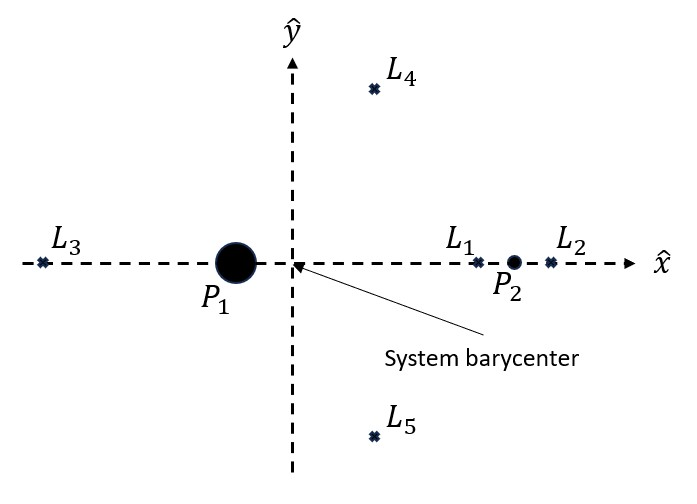
\includegraphics[width=0.5\textwidth]{figures/RotFrame.jpg}
    \caption{CR3BP barycentric rotating frame with Lagrange points.}
    \label{fig:rotFrame}
\end{figure}

\subsection{Jacobi Constant}
One reason that the CR3BP does not have a closed-form analytical solution like the 2BP is there are
not enough integrals of the motion, at least that have been discovered to date. However, there is
one such constant of the motion in the rotating frame, denoted as the Jacobi constant, and it
proves useful as an analogy to energy. The derivation is as follows\cite{Zimovan:2017}:
\begin{equation}
    \nabla U\cdot\rhobardot=\frac{\partial U}{\partial x}\xdot+\frac{\partial U}{\partial y}\ydot+\frac{\partial U}{\partial z}\zdot=(\xddot-2\ydot)\xdot+(\yddot+2\xdot)\ydot+\zddot\zdot,
    \label{eq:JCdotproduct}
\end{equation}
where $\rhobardot$ is the rotating velocity vector. The middle of \cref{eq:JCdotproduct} is
equivalent to the total nondimensional time derivative of the pseudo-potential:
\begin{equation}
    \frac{dU}{d\tau}=\xddot\xdot+\yddot\ydot+\zddot\zdot,
    \label{eq:JCtimeder}
\end{equation}
where $\tau$ is nondimensional time. Integrating and rearranging this equation provides the Jacobi
constant as a function of rotating position and velocity:
\begin{equation}
    C=2U-\rhodot^{2},
    \label{eq:JC}
\end{equation}
where $C$ is the Jacobi constant.

This definition of the Jacobi constant is consistent with the Hamiltonian of the system, which is
time-invariant in the CR3BP\cite{Boudad:2022}. Note also that as the Jacobi constant increases, the
energy of the trajectory decreases.
